\documentclass[10pt,twocolumn,letterpaper]{article}

\usepackage{cvpr}
\usepackage{times}
\usepackage{epsfig}
\usepackage{graphicx}
\usepackage{amsmath}
\usepackage{amssymb}

% Include other packages here, before hyperref.

% If you comment hyperref and then uncomment it, you should delete
% egpaper.aux before re-running latex.  (Or just hit 'q' on the first latex
% run, let it finish, and you should be clear).
\usepackage[breaklinks=true,bookmarks=false]{hyperref}

\cvprfinalcopy % *** Uncomment this line for the final submission

\def\cvprPaperID{****} % *** Enter the CVPR Paper ID here
\def\httilde{\mbox{\tt\raisebox{-.5ex}{\symbol{126}}}}

% Pages are numbered in submission mode, and unnumbered in camera-ready
%\ifcvprfinal\pagestyle{empty}\fi
\setcounter{page}{4321}
\begin{document}

%%%%%%%%% TITLE
\title{Project Proposal for AD4CV: Scan2Cap}

\author{Felix Wimbauer\\
Technical University of Munich\\
{\tt\small felix.wimbauer@tum.de}
% For a paper whose authors are all at the same institution,
% omit the following lines up until the closing ``}''.
% Additional authors and addresses can be added with ``\and'',
% just like the second author.
% To save space, use either the email address or home page, not both
\and
Nicolas Seppich\\
Technical University of Munich\\
{\tt\small nicolas.seppich@tum.De}
}

\maketitle
%\thispagestyle{empty}

%%%%%%%%% ABSTRACT
\begin{abstract}
   The ABSTRACT is to be in fully-justified italicized text, at the top
   of the left-hand column, below the author and affiliation
   information. Use the word ``Abstract'' as the title, in 12-point
   Times, boldface type, centred relative to the column, initially
   capitalized. The abstract is to be in 10-point, single-spaced type.
   Leave two blank lines after the Abstract, then begin the main text.
   Look at previous CVPR abstracts to get a feel for style and length.
   In this work we analyse a pipeline to generate description of 3D scenes using attention methods. 
   
\end{abstract}

%%%%%%%%% BODY TEXT
\section{Introduction}

The "Deep Learning" revolution has enabled great progress in the field of captioning or image description. This task has been studied in a sophisticated way for 2D images using different attention mechanisms.
However, transferring this task to generate a description of an object representation in point clouds or 3D data, there has been no work so far to the best of our knowledge.

Therefore, we are interested in implementing a pipeline to obtain a description for a given object in a 3D scan, using state-of-the-art point cloud feature extractors, object detectors, and a captioning mechanism to generate a semantic description for a given object in the 3D scene. This allows the object to be placed in a global semantic context within its environment.
 
%-------------------------------------------------------------------------
\section{Related Work}
Our work will be based on the ScanRefer dataset \cite{Chen2019}. The dataset consists of 1513 RGB-D scans of ScanNet\cite{Dai2017} 5 unique object descriptions for all existing objects in a scene. The work of \cite{Chen2019} will also be used as guideline in this project.

The extraction of features on point clouds is presented by \cite{Qi2017} applies the feature extraction directly on the point cloud on a hierarchical level, allowing the extraction of local features in a global context. 
The task of object detection on point clouds is studied by \cite{Qi2019}. 

Methods for image captioning using visual attention are described by \cite{Xu2015}, \cite{Lu2016} and \cite{Anderson2017}.
These methods have in common, that they generate a caption for the entire image.
Since our goal includes using a bounding box for the object to be set in context to the scene, the work of \cite{Rohrbach2015} is also of interest for this project. 

%-------------------------------------------------------------------------
\section{Methods and Concept}

Given a point cloud $\mathit{pc \in R^{N\times(d+C)}}$ and an object in that scene, which is described by a target bounding box $b_{target}\in R^6$, our goal is to generate a meaningful caption for the object embedded in the context of the scene. To this end, we plan to use the pipeline described in the following, which was inspired by \cite{Anderson2017}.

To infer information specific to the target object itself, we crop out the points belonging to the bounding box of the object and use a PointNet++ \cite{Qi2017} network on the obtained sub point cloud. This will give a feature vector $\mathit{target\_feats}\in R^{128}$. In order to compute meaningful features, we use weights pretrained for point cloud classification.

To infer information about the scene in general, we employ a VoteNet \cite{Qi2019} network. We don't use the final object labels and bounding boxes, but the feature vectors $\mathit{obj\_feats}\in R^{M\times128}$ generated by the \textit{ProposalModule}.

In our initial pipeline, we combine those features through average pooling into $\mathit{scene\_feats}\in R^{128}$. At a later stage, it is possible to replace this step with attention-based pooling, similar to \cite{Anderson2017}.

For the generation of the caption, we use a classical LSTM. As input, we concatenate the $\mathit{target\_feats}$, $\mathit{scene\_feats}$ and word embedding vector of the previously generated word together. The word embedding is taken from a pre-computed GloVe \cite{pennington2014glove} word embedding matrix. The output of the LSTM is passed through a fully-connected layer and softmax function to obtain probabilities for the various possible next words (similar to \cite{Xu2015}).

\autoref{fig:pipeline} summarizes the project pipeline.

\begin{figure*}
	\centering
	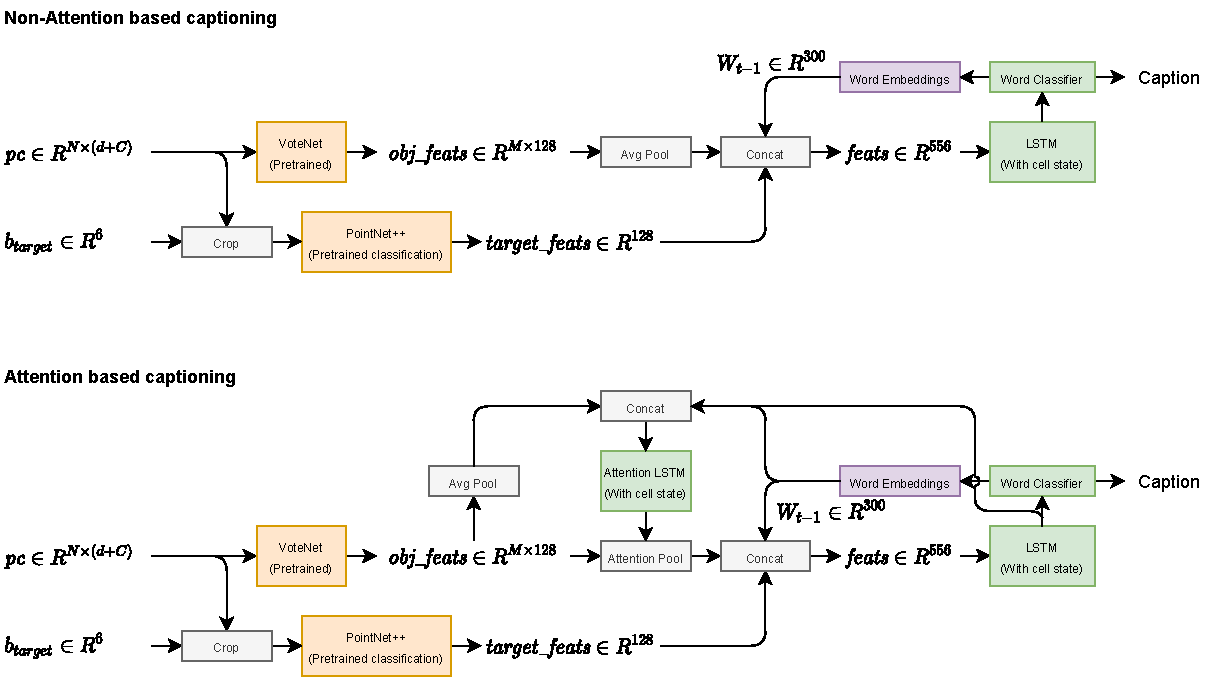
\includegraphics[width=\textwidth]{figures/pipeline_sketch.pdf}
	\caption{Pipeline for project}
	\label{fig:pipeline}
\end{figure*}

{\small
\bibliographystyle{ieee_fullname}
\bibliography{proposal}
}

\end{document}
